% Sinh viên cần nêu rõ các đề tài, sản phẩm liên quan đã được nghiên cứu hoặc đã có trên thị trường trước thời điểm hiện tại và nêu thực trạng của chúng, để từ đó nêu bật được lý do thực hiện nghiên cứu trong KLTN này

Sự phát triển mạnh mẽ của các dịch vụ số như điện toán đám mây, IoT, 5G, trí tuệ nhân tạo và truyền phát video trực tuyến đã làm lưu lượng mạng Internet tăng nhanh, buộc các nhà cung cấp dịch vụ Internet (ISP) phải không ngừng mở rộng hạ tầng và ứng dụng các công nghệ hiện đại như Software-Defined Networking (SDN) để nâng cao hiệu quả quản lý mạng. Tuy nhiên, sự gia tăng lưu lượng cùng tính biến động cao của các ứng dụng hiện đại đã làm phát sinh nhiều vấn đề như tắc nghẽn mạng, mất cân bằng tải, gia tăng độ trễ và suy giảm chất lượng dịch vụ. Trong khi đó, các cơ chế định tuyến và điều khiển lưu lượng chủ yếu dựa trên trạng thái mạng hiện tại thường chỉ phản ứng sau khi lưu lượng thay đổi hoặc tình trạng quá tải bắt đầu xảy ra. Điều này làm hạn chế khả năng chủ động điều chỉnh lưu lượng và phòng tránh tắc nghẽn trước khi xảy ra. Vì vậy, việc nghiên cứu các giải pháp điều khiển lưu lượng có khả năng dự đoán xu hướng lưu lượng trong tương lai và sử dụng thông tin dự đoán để hỗ trợ quyết định Traffic Engineering theo hướng chủ động là cần thiết nhằm nâng cao hiệu quả sử dụng tài nguyên, giảm tắc nghẽn và cải thiện chất lượng dịch vụ trong mạng ISP.

Để giải quyết các vấn đề trên, nhiều giải pháp tối ưu hóa điều khiển lưu lượng đã được nghiên cứu và triển khai như Traffic Engineering, Software-Defined Networking (SDN) và các thuật toán học máy (Machine Learning). Gần đây, các hướng nghiên cứu tập trung vào việc ứng dụng trí tuệ nhân tạo nhằm dự đoán lưu lượng mạng và tối ưu quyết định định tuyến, trong đó Federated Learning (FL) được sử dụng để huấn luyện mô hình dự đoán trên dữ liệu phân tán mà không cần chia sẻ dữ liệu gốc, còn Reinforcement Learning (RL) được áp dụng để học và lựa chọn đường truyền tối ưu theo trạng thái mạng. Tuy nhiên, phần lớn các nghiên cứu hiện nay chỉ tập trung vào từng kỹ thuật riêng lẻ hoặc chưa khai thác hiệu quả sự kết hợp giữa FL và RL trong môi trường mạng ISP dựa trên SDN. Đồng thời, khả năng điều khiển lưu lượng theo hướng chủ động dựa trên dự đoán lưu lượng tương lai vẫn còn là một khoảng trống nghiên cứu cần được tiếp tục khai thác.


\begin{figure}[!h]
    \centering
    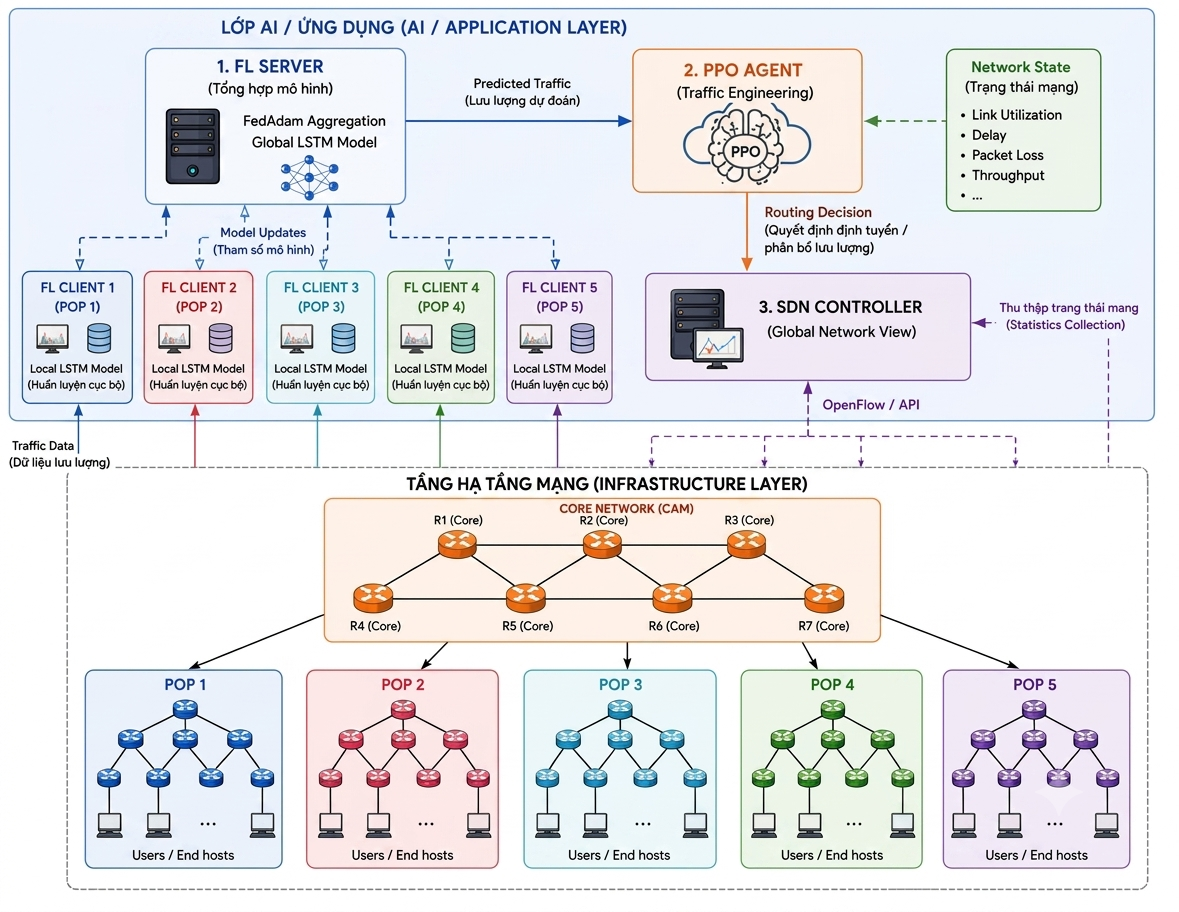
\includegraphics[width=0.75\linewidth]{Figures/Hệ thống đề xuất.png}
    \caption{Hệ thống đề xuất}
    \label{fig:proposed-system}
\end{figure}

Xuất phát từ những hạn chế trên, đề tài đề xuất một giải pháp điều khiển lưu lượng chủ động trong mạng ISP dựa trên SDN bằng cách kết hợp Federated Learning và Reinforcement Learning. Trong kiến trúc đề xuất, FL được sử dụng tại các miền hoặc nút mạng có dữ liệu lưu lượng phân tán để huấn luyện mô hình dự đoán lưu lượng mà không cần tập trung dữ liệu gốc. Các FL Client thực hiện huấn luyện cục bộ và gửi tham số mô hình đến FL Server để tổng hợp thành mô hình toàn cục. Mô hình toàn cục sau đó được sử dụng để dự đoán xu hướng lưu lượng trong tương lai. Kết quả dự đoán được kết hợp với trạng thái mạng hiện tại và cung cấp cho tác tử RL để thực hiện Traffic Engineering, lựa chọn tuyến truyền hoặc phương án phân bổ lưu lượng phù hợp. Quyết định của tác tử RL được chuyển đến bộ điều khiển SDN để thực thi trên các thiết bị mạng, qua đó hướng đến giảm tắc nghẽn, cân bằng tải, cải thiện độ trễ và nâng cao hiệu quả sử dụng tài nguyên mạng.

FL được nghiên cứu nhằm hỗ trợ dự đoán lưu lượng trong các mạng phân tán mà không cần chia sẻ dữ liệu gốc giữa các miền mạng. Li và cộng sự \cite{li2024core} đã kết hợp Vertical Federated Learning và Split Learning để dự đoán lưu lượng mạng lõi, trong khi Gao và cộng sự \cite{gao2024communication} đề xuất cơ chế giảm chi phí truyền thông trong quá trình huấn luyện FL. Zhao và cộng sự \cite{zhao2024federated} áp dụng FL kết hợp Graph Neural Network cho dự đoán lưu lượng trong mạng tích hợp vệ tinh – mặt đất. Tuy nhiên, các nghiên cứu này chủ yếu tập trung vào dự đoán lưu lượng và chưa khai thác kết quả dự đoán để tối ưu quyết định định tuyến.

RL được ứng dụng rộng rãi trong tối ưu định tuyến và điều khiển lưu lượng nhờ khả năng học chính sách tối ưu từ trạng thái mạng. Dake và cộng sự \cite{dake2021traffic} đã tổng quan các phương pháp RL trong Traffic Engineering cho SDN. Al Jameel và cộng sự \cite{aljameel2022reinforcement} sử dụng RL để cải thiện định tuyến cho lưu lượng thời gian thực, trong khi Wang và cộng sự \cite{wang2026deep} kết hợp Deep RL với Graph Multi-Head Attention nhằm nâng cao hiệu quả lựa chọn đường đi. Mặc dù đạt kết quả tốt, các nghiên cứu này chủ yếu dựa trên trạng thái mạng hiện tại và chưa kết hợp thông tin dự đoán lưu lượng để thực hiện điều khiển lưu lượng chủ động.

\begin{table*}[ht]
\centering
\caption{So sánh các công trình nghiên cứu liên quan}
\label{tab:related_work}
\resizebox{\textwidth}{!}{
\begin{tabular}{p{3.2cm}p{3.2cm}p{3.5cm}p{3cm}p{4.8cm}}
\hline
\hline
\textbf{Công trình} &
\textbf{Lĩnh vực} &
\textbf{Hướng tiếp cận} &
\textbf{Mô hình} &
\textbf{Hạn chế} \\
\hline

\citeauthor{li2024core} \cite{li2024core}
&
Traffic Prediction
&
Dự đoán lưu lượng mạng lõi bằng FL
&
Vertical FL + Split Learning
&
Chỉ tập trung dự đoán, chưa tối ưu định tuyến.
\\
\hline

\citeauthor{gao2024communication} \cite{gao2024communication}
&
Traffic Prediction
&
Giảm chi phí truyền thông trong FL
&
Federated Learning
&
Chưa xem xét điều khiển lưu lượng.
\\
\hline

\citeauthor{zhao2024federated} \cite{zhao2024federated}
&
Traffic Prediction
&
Dự đoán lưu lượng mạng di động bằng FL
&
FL + GNN
&
Chưa tích hợp cơ chế định tuyến.
\\
\hline

\citeauthor{aouedi2025deep} \cite{aouedi2025deep}
&
Traffic Prediction
&
Tổng quan các phương pháp DL dự đoán lưu lượng
&
LSTM, GRU, Transformer,...
&
Chỉ tổng hợp nghiên cứu, không đề xuất mô hình mới.
\\
\hline

\citeauthor{dake2021traffic} \cite{dake2021traffic}
&
Traffic Engineering
&
Khảo sát RL trong SDN
&
Q-learning, DQN, PPO,...
&
Không kết hợp dự đoán lưu lượng.
\\
\hline

\citeauthor{aljameel2022reinforcement} \cite{aljameel2022reinforcement}
&
Routing
&
Định tuyến QoS bằng RL
&
Deep Reinforcement Learning
&
Ra quyết định dựa trên trạng thái hiện tại.
\\
\hline

\citeauthor{wang2026deep} \cite{wang2026deep}
&
Routing
&
Tối ưu định tuyến SDN
&
DRL + Graph Attention
&
Chưa sử dụng dự báo lưu lượng.
\\
\hline

\citeauthor{jha2026asynchronous} \cite{jha2026asynchronous}
&
Traffic Engineering
&
Kết hợp FL và RL cho cân bằng tải
&
Federated Reinforcement Learning
&
Tập trung load balancing, chưa nghiên cứu dự đoán lưu lượng.
\\
\hline
\hline
\end{tabular}
}
\end{table*}